\section{Result Evaluation}
\label{sec:result}
In this section, we will analyze the performance of the dynamic hybrid prefetcher. In Fig.\ref{fig:final_acc_cov}, the accuracy and coverage data is displayed. The accuracy performance is similar to the one from \emph{Brute Force Search}, while much less than \emph{ISB}'s and \emph{Static Analysis}'s. The coverage performance is better than the one from \emph{Brute Force Search}, similar to \emph{ISB}'s and \emph{Static Analysis}'s. These are fairly good since before the first 1024 accesses of \emph{ISB} or first 512 accesses of \emph{BO}, the prefetcher acts as a naive hybrid prefetcher.

\begin{figure}[ht!]
   \centering
   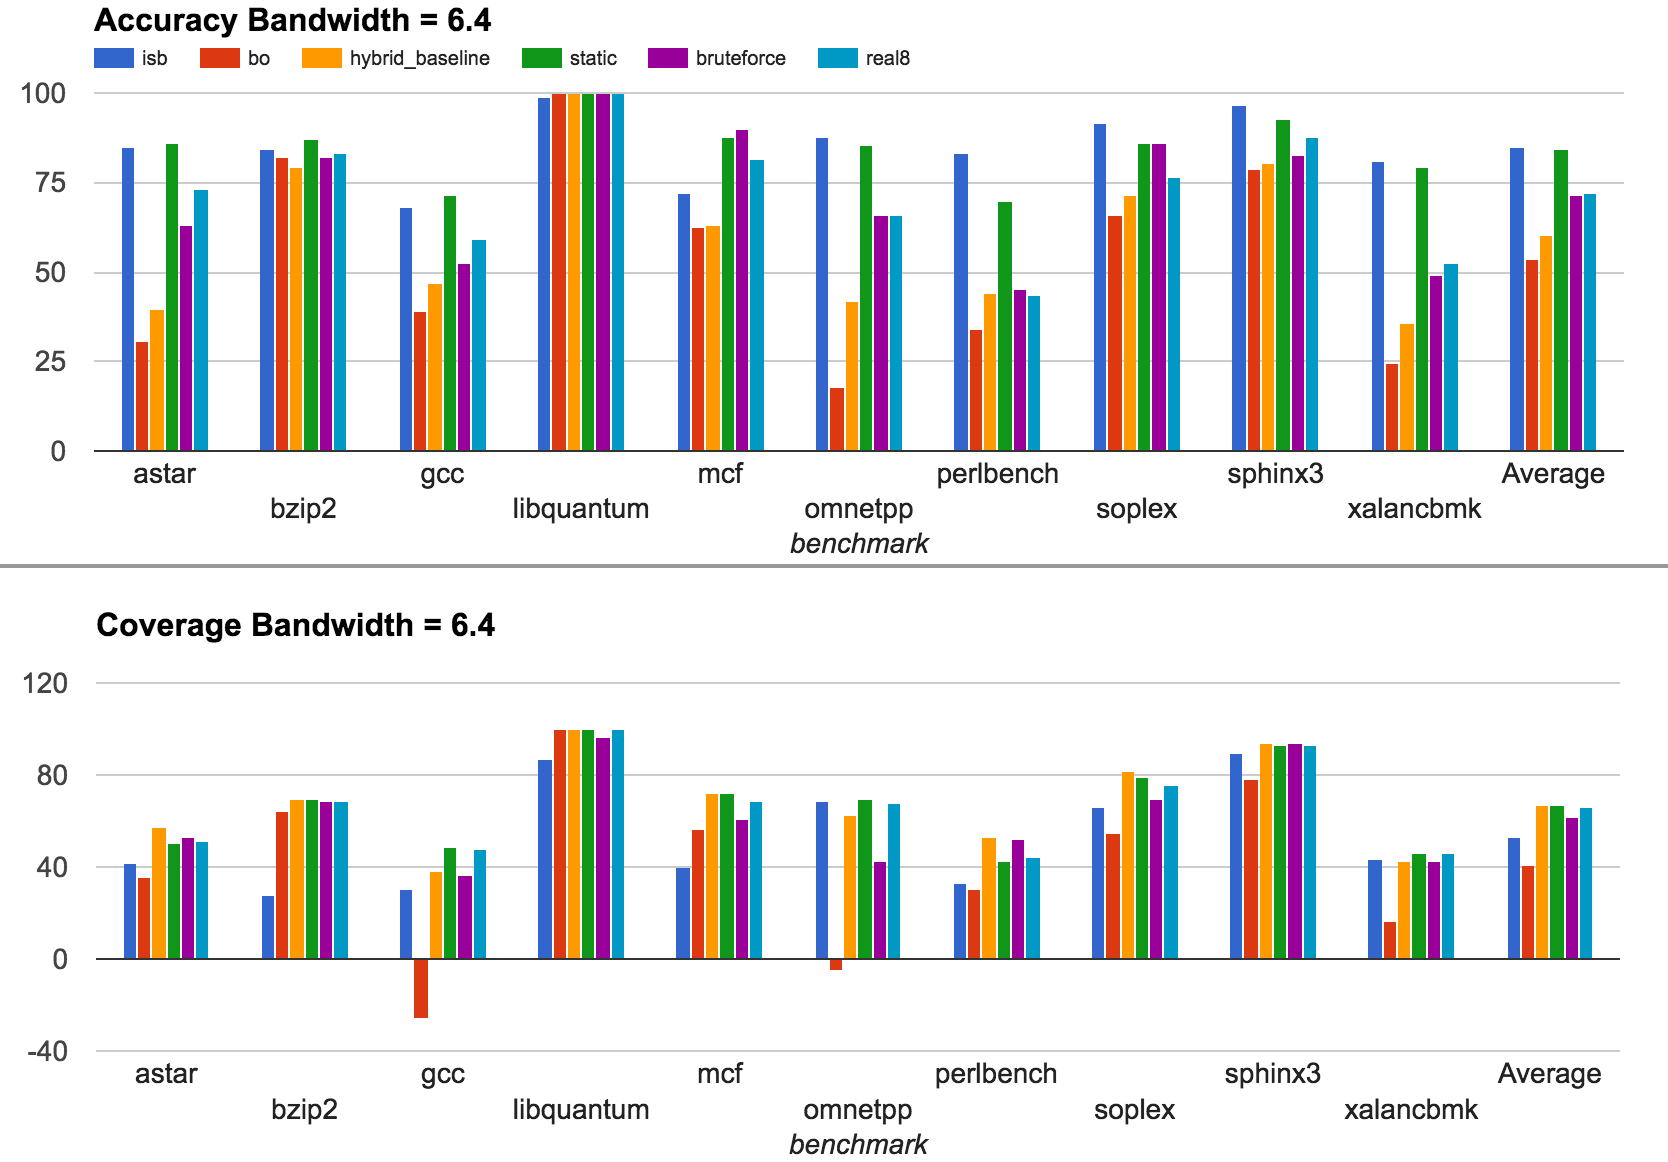
\includegraphics[width=1.0\textwidth]{images/final_acc_cov.png}
   \caption{Accuracy and coverage performance of dynamic hybrid prefetcher}
   \label{fig:final_acc_cov}
\end{figure}

In terms of speedup,

\begin{figure}[ht!]
   \centering
   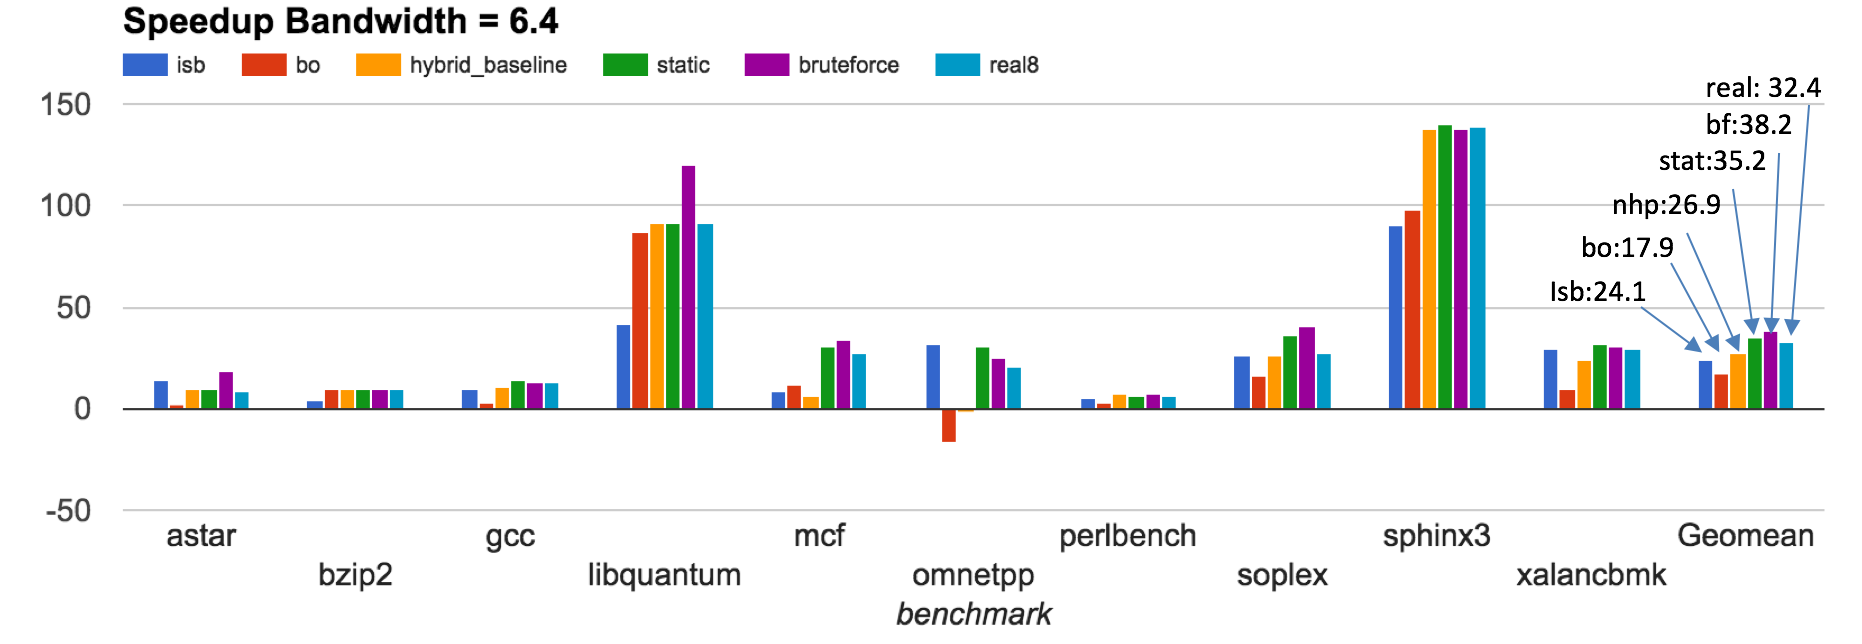
\includegraphics[width=1.0\textwidth]{images/final_speedup.png}
   \caption{Speedup performance of dynamic hybrid prefetcher}
   \label{fig:final_speedup}
\end{figure}

\begin{figure}[ht!]
   \centering
   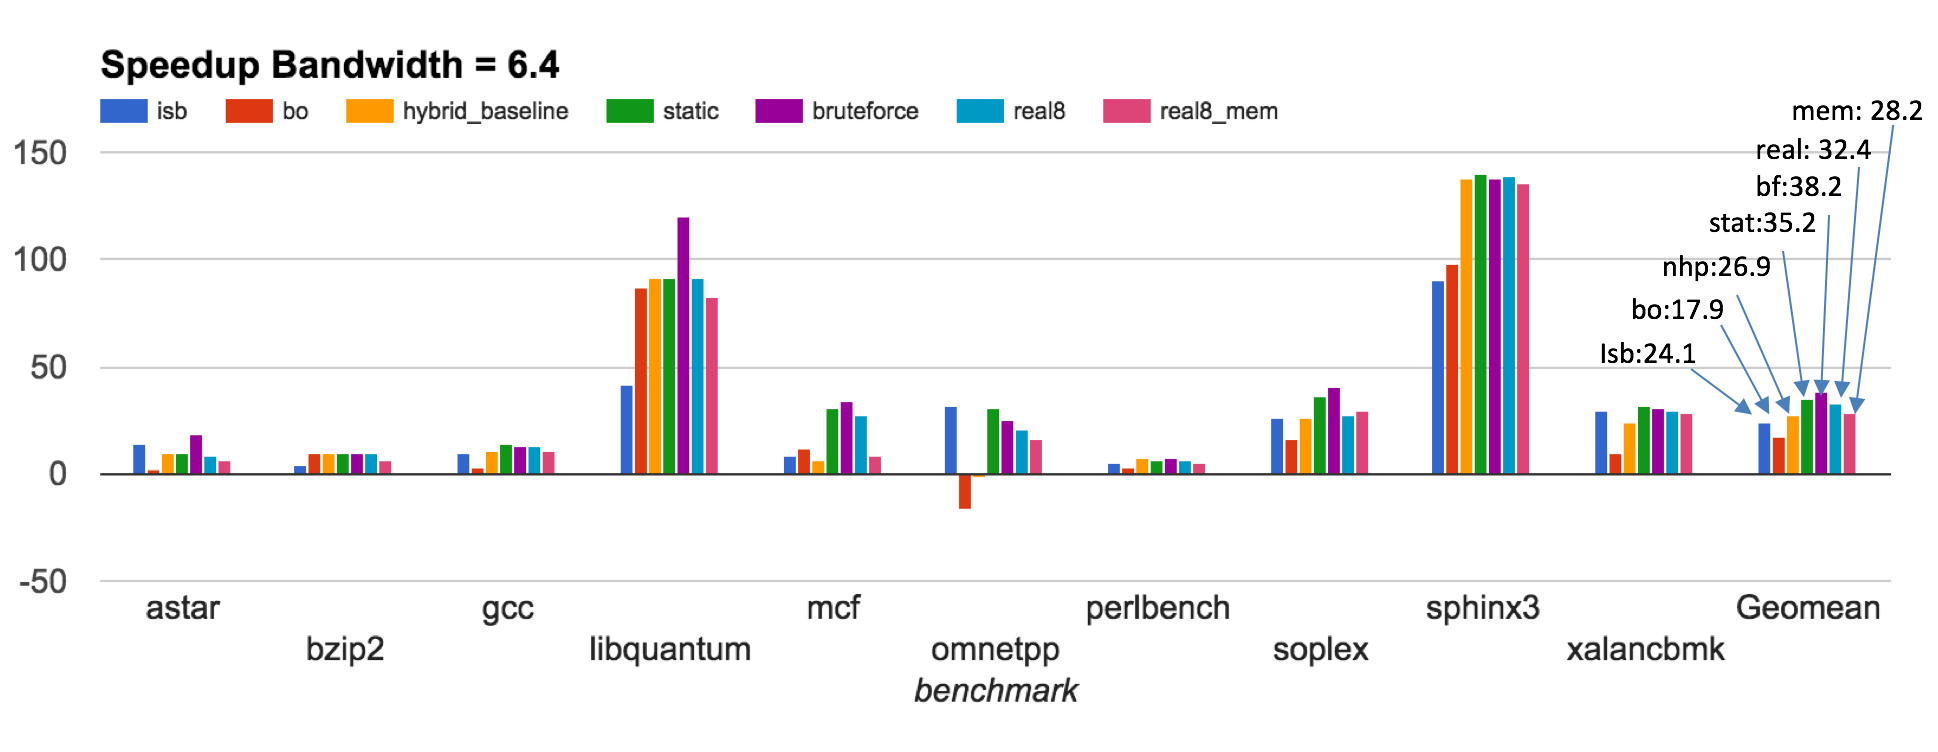
\includegraphics[width=1.0\textwidth]{images/final_speedup_mem.png}
   \caption{Speedup performance of dynamic hybrid prefetcher when consider memory pressure}
   \label{fig:final_speedup_mem}
\end{figure}
